\documentclass[10pt,english]{beamer}
%\documentclass[english,handout]{beamer} % For handouts
\usetheme[progressbar=frametitle,block=fill]{metropolis} %numbering=none

%%% USEFUL PACKAGES
%\usepackage{showframe} % For debugging positioning
\usepackage{etex} % If too many packages
% Encoding and language
\usepackage[utf8]{inputenc}
\usepackage{babel}
\usepackage{amsmath, amssymb}
\usepackage{natbib}
%\usepackage{booktabs}
%\usepackage{algorithmic}
\usepackage{algorithm}
\usepackage{caption}
%\usepackage{animate} % Animations
\usepackage{bm} % Bold math
\usepackage{bbm}
%\usepackage{url}
%\usepackage{pifont}
%\usepackage{ulem} % Used for strikeouts \sout
%\usepackage{stackengine}
%\usepackage{enumitem}
%\setlist[description]{leftmargin=\parindent,labelindent=\parindent}
%\usepackage{colortbl} % Used for colored rows in tables


%%% GRAPHICS
\usepackage{graphicx}
\graphicspath{{./figs/}}


%%% COLORS
\setbeamercolor{background canvas}{bg=white}
\def\BlankFrame{
	\bgroup
	%\pdfpageheight 29.7cm
	\setbeamercolor{background canvas}{bg=}
	\begin{frame}[plain]
	\end{frame}
	%\makeatletter
	%\pdfpageheight \beamer@paperheight
	%\makeatother
	\egroup}

\usepackage{xcolor}
\definecolor{DarkGreen}{HTML}{00B200}
\definecolor{LightBlue}{HTML}{0090D9}
\definecolor{gold}{rgb}{.812,.710,.231}
% Text markup
%\setbeamercolor{alerted text}{fg=red}
\newcommand{\blue}[1]{\textcolor{blue}{#1}}
\newcommand{\red}[1]{\textcolor{red}{#1}}
\newcommand{\grey}[1]{\textcolor{gray}{#1}}
\newcommand{\orange}[1]{\textcolor{mLightBrown}{#1}}
\newcommand\myheading[1]{\textbf{#1}}
\newcommand\myemph[1]{\underline{\emph{#1}}}
\newcommand\textexample[1]{\textit{\textbf{#1}}}

%%% SPACING
\newcommand\vws[1][1]{\vspace{#1\baselineskip}} % vertical white space
%\newcommand\strt[1][1.5ex]{\rule[-.05\baselineskip]{0pt}{#1}} % strut
\newcommand\strt[2]{\rule[-#1ex]{0pt}{#2ex}} % strut
\newcommand\Hrule{\vspace{1ex} \hrule \vspace{1ex}} % Horisontal rule with some space after

%%% MISC
\newcommand\articleref[4]{\noindent\begin{minipage}[t]{0.04\textwidth}
		\vspace{0pt} 
		\pgfuseimage{beamericonarticle}
	\end{minipage}%
	\begin{minipage}[t]{0.96\textwidth}
		\vspace{0pt}
		#1. \textbf{#2.} \textit{#3}, #4.
	\end{minipage}}

%%% METROPOLIS THEME SPECIFIC
\makeatletter
\setlength{\metropolis@progressonsectionpage@linewidth}{1pt}
\makeatother
%\setbeamercolor{progress bar}{fg=red,bg=red!50}


%%% TEXTPOS
\usepackage[absolute,overlay]{textpos} % option showboxes is useful in draft mode
\setlength{\TPHorizModule}{\paperwidth}
\setlength{\TPVertModule}{\paperheight}
\textblockorigin{0pt}{10mm} % start everything at top-left, below gray 


%%% TIKZ/PGFPLOTS
\usepackage{tikz}
\usetikzlibrary{arrows,positioning,calc,shapes.geometric}
%\usetikzlibrary{arrows,calc,shapes.geometric,decorations.pathmorphing,backgrounds,positioning,fit,petri,decorations.pathreplacing}
%\usepackage{pgfplots}
%\pgfplotsset{compat = 1.3}


%%% BLOCKS AND BOXES
% Changing colors of blocks
%\setbeamercolor{block title alerted}{bg=UURed,fg=palette primary.fg}
%\setbeamercolor{block body alerted}{bg=UURed!15}
\setbeamercolor{block title alerted}{bg=mLightBrown,fg=palette primary.fg}
\setbeamercolor{block body alerted}{bg=mLightBrown!15}
%\setbeamercolor{block title example}{bg=UUGreen,fg=palette primary.fg}
%\setbeamercolor{block body example}{bg=UUGreen!10}
% \mybox is a rectangular box
\usepackage{boxedminipage}
\setlength\fboxrule{2pt}
\setlength\fboxsep{2\fboxsep}
\newcommand\mybox[3][\textwidth]{
  {\color{#2}
    \begin{boxedminipage}{#1}
      {\color{palette primary.bg} #3}
    \end{boxedminipage}}%
}   
\usepackage{tcolorbox}
\tcbset{arc=1mm,grow to left by=3mm,grow to right by=3mm,left=2mm}
%\newenvironment{redbox}{%
%	\begin{tcolorbox}[colback=UURed!15,colframe=UURed]}{%
%	\end{tcolorbox}}
%\newenvironment{greenbox}{%
%	\begin{tcolorbox}[colback=UUGreen!15,colframe=UUGreen]}{%
%	\end{tcolorbox}}
\newenvironment{redbox}{%
	\begin{tcolorbox}[colback=red!15,colframe=red]}{%
	\end{tcolorbox}}
\newenvironment{greenbox}{%
	\begin{tcolorbox}[colback=DarkGreen!15,colframe=DarkGreen]}{%
	\end{tcolorbox}}
\newenvironment{graybox}{%
	\begin{tcolorbox}[colback=mDarkTeal!5,colframe=mDarkTeal]}{%
	\end{tcolorbox}}
\newenvironment{orangebox}{%
\begin{tcolorbox}[colback=mLightBrown!15,colframe=mLightBrown]}{%
	\end{tcolorbox}}
\newenvironment{bwbox}{%
	\begin{tcolorbox}[colback=white,colframe=black]}{%
\end{tcolorbox}}
\newenvironment{bluebox}{%
	\begin{tcolorbox}[colback=LightBlue!15,colframe=LightBlue]}{%
\end{tcolorbox}}


%%%%%%%%% NEW MACROS

\newcommand\imp[1]{\alert{\textbf{#1}}}
\newcommand\bfit[1]{\textbf{\textit{#1}}}
\newcommand\good{\color{DarkGreen}{$\blacktriangle$}} % used in lists
\newcommand\bad{\color{red}{$\blacktriangledown$}} % used in lists


\RequirePackage{amsmath, amssymb}
\RequirePackage{bbm}
%\RequirePackage{newtxmath}


% Convenience macro for referring to data source
\newcommand\sourceurl[2]{\small \grey{Data from \href{#1}{#2}}}

% Abbreviations
\RequirePackage{xspace}
\newcommand\pdf{pdf\xspace}
\newcommand\ifft{iff\xspace}
\newcommand\ex{\textbf{ex)}\xspace}

% General time series notation
\newcommand\T{n}  % Length of time series
\newcommand\rtheta{{\red{\theta}}}  % Parameter (color coded)
\newcommand\rthetah{{\red{\widehat\theta}}}  % Estimate (color coded)

% Neural netowkrs
\newcommand\h{\mathbf{h}} % Hidden state variable
\newcommand\zz{\mathbf{z}} % Generic input (vector)

% For OLS/AR
\newcommand\noise{\varepsilon}  % This is the noise in AR, but should it be the same as measurement noise in SSM?
\newcommand\noisevar{\sigma^2_\noise}
\newcommand\noisevarhat{\widehat\sigma^2_\noise}
\newcommand\X{\Phi}
\newcommand\y{\mathbf{y}}
\newcommand\bphi{\bm\phi}

% State space models
\newcommand\z{\alpha}  % State vector, general SSM
\newcommand{\obsnoise}{\varepsilon}
\newcommand{\statenoise}{\eta}
\newcommand{\varobs}{\sigma^2_{\varepsilon}}
\newcommand{\varstate}{\sigma^2_{\eta}}
% For structural time series
\newcommand{\trendnoise}{\zeta}
\newcommand{\seasnoise}{\omega}
\newcommand{\vartrend}{\sigma^2_{\trendnoise}}
\newcommand{\varseas}{\sigma^2_{\seasnoise}}

%
\newcommand\FF{T}
\newcommand\GG{R}
\newcommand\HH{Z}
\newcommand{\covobs}{\sigma_\epsilon^2}
\newcommand{\covstate}{Q}
\newcommand\initmean{a_1}
\newcommand\initcov{P_1}
% Kalman filter
\newcommand{\zpart}[2]{\z_{#1}^{#2}}
\newcommand{\wgt}[2]{\omega_{#1}^{#2}}
\newcommand{\wgtsum}[1]{\Omega_{#1}}
\newcommand\zhat[2]{\hat\z_{#1|#2}}
\newcommand\Phat[2]{P_{#1|#2}}
\newcommand\zpred[1]{\zhat{#1}{#1-1}}
\newcommand\Ppred[1]{\Phat{#1}{#1-1}}
\newcommand\zfilt[1]{\zhat{#1}{#1}}
\newcommand\Pfilt[1]{\Phat{#1}{#1}}
\newcommand\ypred[1]{\hat y_{#1|#1-1}}
\newcommand\Spred[1]{F_{#1|#1-1}}
\newcommand\Spredinv[1]{\Spred{#1}^{-1}}
\newcommand\epshat[2]{\hat{\obsnoise}_{#1|#2}}
\newcommand\etahat[2]{\hat{\statenoise}_{#1|#2}}

\newcommand{\statefun}{T}
\newcommand{\obsfun}{Z}
\newcommand{\estfun}{h}

\newcommand{\qd}{q} %State density
\newcommand{\md}{g} %Measure density

\newcommand{\rmd}{\mathrm{d}}

% SMC
\newcommand{\Np}{N}           % Number of particles
\newcommand{\Mp}{M}           % Number of particles in backward simulation



%\RequirePackage{color}
%\newcommand{\flnote}[1]{{\color{red}\textbf{[#1]}}} % Used for notes in text - color red
%\newcommand\Hrule{\vspace{1ex} \hrule \vspace{1ex}} % Horisontal rule with some space after; This is moved to beamer preamble

%%%%%%%%%%%%%%%%%%%%%%%%%%%%%%%%%%%%%%%%%%%%%%%%%%%%%%%%%%%%%%%%%%%%%%%%%%%%%%%%
%                            COMMANDS IN TEXT                                  %
%%%%%%%%%%%%%%%%%%%%%%%%%%%%%%%%%%%%%%%%%%%%%%%%%%%%%%%%%%%%%%%%%%%%%%%%%%%%%%%%
\newcommand\numtext[2]{#1\textsuperscript{#2}}
\newcommand\thsnd[1]{\ensuremath{#1\thinspace000}}
\newcommand{\peqref}[1]{\eqref{#1} on page~\pageref{#1}} % Page referencing for equations: "(1) on page 1"

%%%%%%%%%%%%%%%%%%%%%%%%%%%%%%%%%%%%%%%%%%%%%%%%%%%%%%%%%%%%%%%%%%%%%%%%%%%%%%%%
%                            SPECIFIC MATH                                     %
%%%%%%%%%%%%%%%%%%%%%%%%%%%%%%%%%%%%%%%%%%%%%%%%%%%%%%%%%%%%%%%%%%%%%%%%%%%%%%%%
% Models etc.
%\newcommand{\T}{T}            % Number of samples in data record
\newcommand{\parspace}{\Theta}                                   % Parameter space
\newcommand{\parameter}{\theta}                                  % Parameter
% Spaces
\newcommand{\setX}{\ensuremath{\mathsf{X}}}                      % State-space X
\newcommand{\sigmaX}{\ensuremath{\mathcal{X}}}                   % Sigma algebra on X
\newcommand{\setY}{\ensuremath{\mathsf{Y}}}                      % State-space Y
\newcommand{\sigmaY}{\ensuremath{\mathcal{Y}}}                   % Sigma algebra on Y
\newcommand{\setZ}{\ensuremath{\mathsf{Z}}}                      % State-space Z
\newcommand{\sigmaZ}{\ensuremath{\mathcal{Z}}}                   % Sigma algebra on Z

%%%%%%%%%%%%%%%%%%%%%%%%%%%%%%%%%%%%%%%%%%%%%%%%%%%%%%%%%%%%%%%%%%%%%%%%%%%%%%%%
%                           GENERAL MATH                                       %
%%%%%%%%%%%%%%%%%%%%%%%%%%%%%%%%%%%%%%%%%%%%%%%%%%%%%%%%%%%%%%%%%%%%%%%%%%%%%%%%

% ======== Miscellaneous symbols ========
\newcommand\eqdef{:=}
\newcommand\defeq{=:}
\newcommand\const{\text{const.}}
%\newcommand\eqdef{\stackrel{\text{\scriptsize def}}{=}}

\newcommand\iid{iid}
\newcommand{\iidsim}{\stackrel{\text{\iid}}{\sim}} % iid simulation
\newcommand{\process}[1]{\{#1\}_{t\geq 1}}       % Process (time index t)
\newcommand{\range}[2]{#1, \, \dots, \, #2}      % Range = 1, ..., N
\newcommand{\crange}[2]{\{#1, \, \dots, \, #2\}} % Curly range = {1, ..., N}
\newcommand{\prange}[2]{(#1, \, \dots, \, #2)}   % Parenthesised range = (1, ..., N)
\newcommand{\bwdrange}[2]{#1 : -1 : #2}          % Range = N, ..., 1
\newcommand{\approxpropto}{\stackrel{\sim}\propto}

% Tight dots between \int and \int in a multidimensional integral
\newcommand{\tightcdots}{\hspace*{-0.38em}\cdot\hspace*{-0.3em}\cdot\hspace*{-0.3em}\cdot\hspace*{-0.38em}}

% Arrows - convergence and mappings
% \mapsto                                                     % Mappings, x \mapsto f(x)
\newcommand{\fromto}{\rightarrow}                             % Mapping from set A to set B; f: A \fromto B
\newcommand{\goesto}{\rightarrow}                             % limits used in n \goesto \infty
\newcommand{\goestosmall}{\to}                                % limits used in \lim_{n \goestosmall \infty}
\newcommand{\convP}{\stackrel{\probab}\longrightarrow}        % Convergence in probability
\newcommand{\convD}{\stackrel{\textrm{D}}\longrightarrow}     % Convergence in distribution

% ======== Standard spaces  ========
\newcommand{\naturals}{\ensuremath{\mathbb{N}}}               % Natural numbers
\newcommand{\reals}{\ensuremath{\mathbb{R}}}                  % Real numbers
\newcommand{\nonnegatives}{\reals_{\smaller +}}               % Nonnegative numbers
\newcommand{\positives}{\reals_{\smaller ++}}                 % Positive numbers
\newcommand{\nonnegativedefinites}[1]{S_{\smaller +}(#1)}     % Nonnegative #1 x #1 matrices
\newcommand{\positivedefinites}[1]{S_{++}(#1)}                % Positive #1 x #1 matrices

% ======== Matrices ========
\newcommand{\eye}[1]{I_{#1}}                     % Identity matrix
\newcommand{\+}{\mathsf{T}}                      % Transpose
\newcommand{\kronecker}{\raisebox{1pt}{\ensuremath{\otimes}}} % Kronecker product
\DeclareMathOperator*\diag{diag}
\DeclareMathOperator*\trace{tr}

% ======== Operators, calculus etc. ========
\newcommand{\Ordo}{O}                            % Big ordo
\newcommand{\supnorm}[1]{\|#1\|_\infty}          % Supremum norm
\newcommand\osc{\text{osc}}                      % Oscillator norm
\newcommand{\grad}{\nabla}                       % Gradient
\newcommand{\complementof}[1]{\ensuremath{#1^\mathsf{c}}} % Set complement
\renewcommand\vec{\text{vec}}
\DeclareMathOperator*\supp{supp}                          % Support
\DeclareMathOperator*\card{card}                          % Set cardinality
\DeclareMathOperator*\rank{rank}                          % Rank
\DeclareMathOperator*\sign{sign}                          % Signum function
\DeclareMathOperator*\argmax{arg\,max}
\DeclareMathOperator*\argmin{arg\,min}

% ======== Probability ========
\newcommand{\Prb}{\ensuremath{\mathbb{P}}}                       % Probability
\newcommand{\E}{\ensuremath{\mathbb{E}}}                         % Expectation
\newcommand{\var}{\ensuremath{\mathrm{Var}}}                     % Variance
\newcommand{\cov}{\ensuremath{\mathrm{Cov}}}                     % Covariance
\newcommand{\cor}{\ensuremath{\mathrm{Corr}}}                     % Correlation
\newcommand{\I}{\ensuremath{\mathbbm{1}}}						 % Indicator function

%\newcommand{\abscont}{\ensuremath{\ll}}          % Absolute continuity
\renewcommand\mid{\,\vert\,} % I don't really like that \mid produces rubber lengths. Sometimes, we get very large white spaces p(x    |   y), and it can produce line breaks after "p(x |" . Is the non-rubber definition here better?
\newcommand\Mid{\,\middle\vert\,} % Stretchable |, to use with \left \right - N.B. This produces a longer | in general. Does that look better than a standard \mid?


% Distributions
\newcommand{\N}{\ensuremath{\mathcal{N}}}        % Normal
\newcommand{\uni}{\ensuremath{\mathcal{U}}}      % Uniform
\newcommand\MN{\mathcal{MN}}                     % Matrix normal
\newcommand\IW{\mathcal{IW}}                     % Inverse-Wishart
\newcommand\GP{\mathcal{GP}}                     % Gaussian process
\DeclareMathOperator*\Mult{Mult}                 % Multinomial
\DeclareMathOperator*\cat{Cat}                   % Categorical
\DeclareMathOperator*\Discrete{Discrete}         % Categorical/alternative name
\DeclareMathOperator*\bin{Bin}                   % Binomial
\DeclareMathOperator*\gam{Gam}                   % Gamma
\DeclareMathOperator*\St{St}                     % Student's t
\DeclareMathOperator*\po{Po}                   % Binomial

%\usepackage{extendedalt}
%\usepackage{animate} % Animations
%\usepackage{../lindsten}
%\usepackage{movie15}
\usepackage{tikz}
\usepackage{listofitems} % for \readlist to create arrays

\hypersetup{
  colorlinks=true, urlcolor=blue, linkcolor=red
}

\title{732G57 Maskininlärning för statistiker}
\subtitle{Föreläsning 11}
\date{}
\author{Josef Wilzén \\ IDA, Linköping University, Sweden}
\titlegraphic{\hfill
\includegraphics[height=1.2cm]{../LiU_primary_black.pdf}}
%\institute{Joint work with\dots}


%% MY DEF %%
\newcommand{\itm}[1]{\mathrm{Item}_{#1}}
\newcommand{\pausa}{\pause}
%\renewcommand{\pausa}{}
\tikzstyle{mynode}=[thick,draw=blue,fill=blue!20,circle,minimum size=22]


\newenvironment{nscenter}
 {\parskip=0pt\par\nopagebreak\centering}
 {\par\noindent\ignorespacesafterend}

\begin{document}

\maketitle

\begin{frame}{Dagens föreläsning}

    \begin{itemize}
        \item Info
        \item Del 1:
        \begin{itemize}
          \item Datahantering
          \item Modellering, modellval, hyperparametrar  
        \end{itemize}
        \item Del 2:
        \begin{itemize}
          \item Lite från gamla föreläsningar
          \item Utblickar - tillämpningar och utökningar inom ML
          \item Sammanfattning av kursen
        \end{itemize}
    \end{itemize}
    
\end{frame}

\begin{frame}{Projekt och resten av kursen}
    
  \begin{itemize}
        \item Kursvecka 7 och framåt: 
        \begin{itemize}
          \item Arbeta med projektet
          \item Datorlabbar: hjälp med projektet $\rightarrow$ utnyttja tiden!
          \item Förbereda inför tentan
        \end{itemize}
        \item Datum: \href{https://raw.githubusercontent.com/STIMALiU/732G57_ML/refs/heads/main/project/Datum_ht2025.pdf}{länk}
    \end{itemize}

\end{frame}


\begin{frame}{Välja kurser till vårterminen}
  Till VT så ska ni välja kurser på 15 HP. \\
  Några rekommendationer om man är intresserad av maskininlärning.
  \begin{itemize}
        \item Det viktigaste är att välja en kurs som man är motiverad att läsa!
        \item Om man vill arbeta direkt efter examen: 
        \begin{itemize}
          \item Läs en kurs i programmering i Python
        \end{itemize}
        \item Om man är intresserad av master i \href{https://liu.se/en/education/program/f7mml}{Statistics and Machine Learning}
         \begin{itemize}
          \item \href{https://studieinfo.liu.se/kurs/764G03\#examination}{764G03 Flervariabelanalys}
          \item Någon grundkurs i optimering
          \item Python/Fördjupande kurs i programmering/algoritmer/datastrukturer
        \end{itemize}
    \end{itemize}

\end{frame}


\begin{frame}[standout]
    \LARGE Del 1: \\ Datahantering och Modellering
\end{frame}



\begin{frame}{Förstå och förbered data}
\begin{itemize}
    \item Identifiera förklarande variabler och responsvariabel.
    \item Beskriv vad som utgör en observation i datasetet.
    \item Hantera kategoriska variabler – slå ihop obalanserade kategorier vid behov.
    \item Undersök extremvärden – uteslut endast med tydliga regler.
    \item Hantera saknade värden:
    \begin{itemize}
        \item Uteslutning är ofta enklast.
        \item Imputering kan användas, men med försiktighet.
    \end{itemize}
\end{itemize}
\end{frame}


\begin{frame}{Dela upp data}
\begin{itemize}
    \item Dela upp i:
    \begin{itemize}
        \item Träningsdata
        \item Valideringsdata
        \item Testdata
    \end{itemize}
    \item Vid klassificering: kontrollera klassfördelning i alla dataset.
    \item Testdata används först i slutet för att skatta framtida testfel (generaliserbarhet).
\end{itemize}
\end{frame}

\begin{frame}{Standardisering och transformationer}
\begin{itemize}
    \item Standardisera kontinuerliga variabler vid behov.
    \item Spara \texttt{x\_mean\_train} och \texttt{x\_sd\_train} för varje kontinuerlig variabel.
    \item Använd dessa värden för att standardisera validerings- och testdata.
    \item De flesta problem kräver att vi gör en viss mängd manuella 
    transformationer av vissa variabler (feature engingering).
    \item Ibland behöver vi transformera responsvariabeln, ex: $y_{log} = log(y)$
    \item Transformationer bör baseras på träningsdata
    \begin{itemize}
        \item Ex: log-transformera variabler.
        \item Ex: skapa kategorier utifrån medianvärde i träningsdata.
    \end{itemize}
\end{itemize}
\end{frame}

\begin{frame}{Praktiskt arbetssätt}
\begin{itemize}
    \item Börja med en kort explorativ fas för att förstå data och möjliga metoder.
    \item Formulera ett strukturerat upplägg:
    \begin{itemize}
        \item Hur ska data delas upp?
        \item Vilka modeller ska användas?
        \item Vilka hyperparametrar ska testas?
    \end{itemize}
    \item Beskriv detta upplägg tydligt i rapportens metoddel, under Praktisk Metod.
\end{itemize}
\end{frame}



\begin{frame}{Hyperparametrar – val och optimering}
\begin{itemize}
    \item Vissa hyperparametrar fixeras (tidsbegränsningar, avgränsning).
    \item Andra optimeras med hjälp av valideringsdata eller korsvalidering.
    \item Viktiga hyperparametrar bör identifieras via litteratur.
    \item Ange tydligt:
    \begin{itemize}
        \item Vad som fixeras
        \item Vad som optimeras
        \item Vilka värden som testas
        \item Vilka mått som används för utvärdering
    \end{itemize}
\end{itemize}
\end{frame}


\begin{frame}{Loopar för hyperparametersökning}
\begin{itemize}
    \item Skatta flera modeller genom att loopa över vektor/lista med hyperparametervärden
    \item Spara resultat för träning och validering i vektorer/matriser.
    \item Jämför modeller baserat på utvärderingsmått.
    \item Exempel:
    \begin{itemize}
        \item Testa olika värden på \texttt{k} i KNN.
        \item Välj det \texttt{k} som ger lägst genomsnittligt MSE på valideringsdata.
    \end{itemize}
\end{itemize}
\end{frame}


\begin{frame}{Utvärdering av modeller}
\begin{itemize}
    \item Hur ska modellerna utvärderas och jämföras?
    \item Välj lämpliga utvärderingsmått:
    \begin{itemize}
        \item Klassificering: övergripande och klassvisa mått
        \item Regression: övergripande mått och residualanalys
    \end{itemize}
    \item Visualisera resultat med plottar och tabeller.
\end{itemize}
\end{frame}

\begin{frame}{Val av utvärderingsmått}
\begin{itemize}
    \item \textbf{Klassificering:}
    \begin{itemize}
        \item Övergripande mått: Träffsäkerhet, felkvot
        \item Klassvisa mått: Sensitivitet, Specificitet, Precision, F1-score
        \begin{itemize}
          \item Viktigt vid \textbf{obalanserade} klasser
        \end{itemize}
    \end{itemize}
    \item \textbf{Regression:}
    \begin{itemize}
        \item Övergripande mått: MSE, MAE 
        \item Residualanalys: undersök systematiska fel
        \item MAE kan vara bättre än MSE vid extrema värden i residualerna
    \end{itemize}
\end{itemize}
\end{frame}

\begin{frame}{Klassobalans i klassificering}
\begin{itemize}
    \item Vid tydlig obalans i responsvariabeln kan följande metoder användas:
    \begin{itemize}
        \item \textbf{Undersampling:} Minska antalet observationer i majoritetsklassen.
        \item \textbf{Oversampling:} Öka antalet observationer i minoritetsklassen, t.ex. genom duplicering eller syntetiska exempel (SMOTE).
        \item \textbf{Viktade kostnadsfunktioner:} Ge högre vikt till minoritetsklassen vid träning.
        \begin{itemize}
            \item Exempel: viktad MSE, viktad cross-entropy loss
        \end{itemize}
    \end{itemize}
    \item Syftet är att förbättra modellens förmåga att identifiera minoritetsklassen.
    \item Se kap 6.11 i \textbf{IDM}
\end{itemize}
\end{frame}

\begin{frame}{Användning av valideringsdata}
\begin{itemize}
    \item Valideringsdata används för att välja hyperparametrar.
    \item Oftast väljer vi den modell som ger lägst fel på valideringsdata givet valda utvärderingsmått
    \item När bästa kombinationen hyperparametrar hittats för en modell:
    \begin{itemize}
        \item Skatta om modellen med träningsdata \textbf{och} valideringsdata.
        \item Antagande: bra hyperparametrar → rimlig regularisering.
        \item Mer data kan användas utan att riskera överanpassning.
    \end{itemize}
\end{itemize}
\end{frame}



\begin{frame}{Nästlade valideringsscheman}
\begin{itemize}
    \item Ibland skapas en extra valideringsmängd inom träningsdata.
    \item Används för att välja hyperparametrar för en specifik modellklass.
    \item Kräver att man har tillräckligt mycket data.
    \item Exempel: intern validering i Keras vid träning av neurala nätverk.
\end{itemize}
\end{frame}


\begin{frame}{Exempel – lasso vs neurala nätverk}
\begin{itemize}
    \item Dela upp data i träning, validering och test.
    \item \textbf{Lasso regression:}
    \begin{itemize}
        \item Använd korsvalidering på träningsdata för att välja $\lambda$.
    \end{itemize}
    \item \textbf{Neurala nätverk:}
    \begin{itemize}
        \item Skapa intern valideringsmängd inom träningsdata.
        \item Välj hyperparametrar för nätverket, exempel:
        \begin{itemize}
          \item antal gömda lager, antal noder i lager
          \item learning rate, batch size
        \end{itemize}
    \end{itemize}
    \item Jämför modeller på valideringsdata.
    \item Välj bästa modell och utvärdera på testdata.
\end{itemize}
\end{frame}


\begin{frame}{Projektet - resultat}
\begin{itemize}
    \item Använd tydliga tabeller för att visa mått för olika modeller/hyperparametervärden
    \item Presentera resultat för både träningsdata och valideringsdata \\ (i samma tabell)
    \item Plottar kan exempelvis användas för att illustrera:
    \begin{itemize}
        \item Modellens prestanda över skattningsiterationer
        \item Effekten av olika förklarande variabler
        \item Residualer (vid regression)
    \end{itemize}
\end{itemize}
\end{frame}


\begin{frame}{Revidering av upplägg}
\begin{itemize}
    \item Det är tillåtet att revidera sitt praktiska upplägg under analysens gång. 
    \item Viktigt att uppdatera beskrivningen av upplägget i rapporten.
    \item Exempel på revidering:
    \begin{itemize}
        \item Ändrad datadelning
        \item Ny modellklass
        \item Justerade hyperparametrar
    \end{itemize}
\end{itemize}
\end{frame}


\begin{frame}{Tolkningsbarhet vs prediktiv förmåga}
\begin{itemize}
    \item Modeller skiljer sig i hur lätta de är att tolka och hur bra de är på prediktioner.
    \item \textbf{Mer tolkningsbara:}
    \begin{itemize}
        \item Linjär regression, logistisk regression
        \item Grunda trädmodeller, Generalized Additive Models (GAM)
    \end{itemize}
    \item \textbf{Mellanläge:}
    \begin{itemize}
        \item Djupare träd, Random Forest, Boosting
    \end{itemize}
    \item \textbf{Mindre tolkningsbara:}
    \begin{itemize}
        \item Neurala nätverk, KNN
    \end{itemize}
    \item Valet beror på syftet: förklaring eller prediktion?
\end{itemize}
\end{frame}

\begin{frame}{Tolkningsbarhet vs Prediktiv förmåga}
Konceptuell bild över olika modellers egenskaper.
\begin{figure}
    \centering
    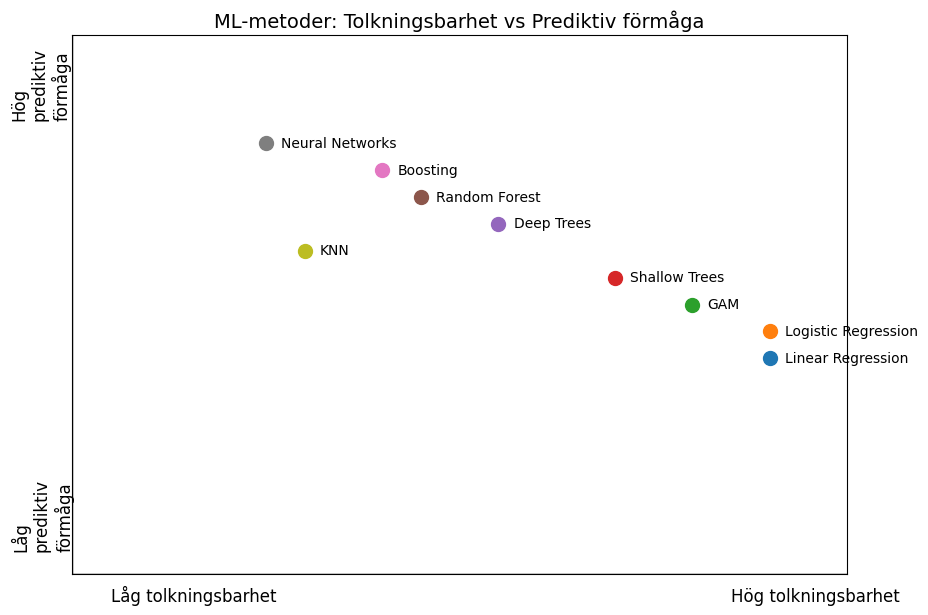
\includegraphics[width=0.8\linewidth]{ml_methods_interpretability_vs_predictive_power3.png}
\end{figure}
\end{frame}


\begin{frame}[standout]
    \LARGE Del 2: \\ Sammanfattning av kursen, \\ utblickar mm
\end{frame}


\begin{frame}{Rester från tidigare föreläsningar}
\begin{itemize}
    \item Autoencoders
    \item XGBoost
\end{itemize}
\end{frame}

\begin{frame}{Utblickar inom maskininlärning}
  \begin{itemize}
    \item Kursen fokuserar på grundläggande ML-metoder
    \item Det finns många avancerade och specialiserade metoder
    \item Här följer några exempel på utökningar och utblickar
  \end{itemize}
\end{frame}

\begin{frame}{Probabilistisk ML – Flexibel modellering}
  \begin{itemize}
    \item Modellera \textbf{alla parametrar} i likelihoodfunktionen med flexibla funktioner
    \item Går bortom antagandet om konstant varians eller fixerad form
    \item \textbf{Normalfördelning}: modellera både medelvärde och varians som funktioner av indata
    \item \textbf{Poissonfördelning}: modellera intensitet ($±\lambda$) för räknevariabler
    \item \textbf{Gammafördelning} och \textbf{Log-normalfördelning}: \\ modellera respons: $y\in \mathbb{R}^+$
    \item \textbf{Quantile regression}: modellera olika kvantiler direkt, utan antagande om fördelning
  \end{itemize}
\end{frame}


\begin{frame}{Normal likelihood med neurala nätverk}
  Antag att vi har $n$ observationer $(x_i, y_i)$ för $i = 1, \dots, n$. Vi modellerar:
  \[
  y_i \mid x_i \sim \mathcal{N}(\mu(x_i), \sigma^2(x_i))
  \]
  där:
  \[
  \mu(x_i) = f_\mu(x_i; \theta_\mu), \quad \log \sigma^2(x_i) = f_\sigma(x_i; \theta_\sigma)
  \]
  Den totala log-likelihood ges av:
  \[
  \log p(y_1, \dots, y_n \mid x_1, \dots, x_n) = 
  -\frac{1}{2} \sum_{i=1}^n \left[ \log(2\pi \sigma^2(x_i)) + \frac{(y_i - \mu(x_i))^2}{\sigma^2(x_i)} \right]
  \]
  \begin{itemize}
    \item Två separata nätverk för $\mu(x)$ och $\sigma^2(x)$
    \item Träning sker genom att maximera log-likelihood över hela datasetet
  \end{itemize}
\end{frame}

\begin{frame}{Bayesianska metoder}
  \begin{itemize}
    \item Modellering med sannolikhetsfördelningar
    \item Ger osäkerhetsmått och möjliggör inferens
    \item Baseras på Bayes sats: $p(\theta |y,X) \propto p(y|\theta,X) \cdot p(\theta)$
    \item Generellt ramverk för inferens som kan användas för traditionella metoder och inom ML
    \item Exempel: Bayesiansk regression, Gaussian Processes regression, BART, Bayesian Deep Learning
    \item Kräver ofta MCMC eller variational inference
    \item Se kursen  \href{https://studieinfo.liu.se/kurs/732G43}{732G43 Bayesiansk statistik}
  \end{itemize}
\end{frame}

\begin{frame}{Tidserieprognoser med maskininlärning}
  \begin{itemize}
    \item ML-modeller kan användas för att förutsäga framtida värden i en tidsserie
    \item Kräver ofta att data omvandlas till ett övervakat format:
    \[
    \text{Input: } (y_{t-1}, y_{t-2}, \dots, x_{t-1}, x_{t-2}, \dots), \quad \text{Output: } y_t
    \]
    \item Exempel på ML-metoder:
    \begin{itemize}
      \item Trädmodeller (t.ex. XGBoost)
      \item Neurala nätverk (t.ex. MLP, LSTM)
      \item Hybridmodeller: ML + ARIMA
    \end{itemize}
    \item Fördelar: kan hantera icke-linjära samband och flera indata
    \item Utmaningar: sekventiellt beroende, överanpassning, databehandling
  \end{itemize}
\end{frame}

\begin{frame}{Tolkningsbar maskininlärning}
  \begin{itemize}
    \item Målet: förstå hur och varför en modell gör sina prediktioner
    \item Viktigt inom känsliga tillämpningar: medicin, juridik, finans
    \item Exempel på metoder:
    \begin{itemize}
      \item Feature importance (t.ex. permutation, SHAP)
      \item Partial dependence plots (PDP)
      \item Surrogatmodeller (t.ex. träd som approximerar komplexa modeller)
      \item Lokala förklaringar (t.ex. LIME)
    \end{itemize}
    \item Rekommenderad läsning: \href{https://christophm.github.io/interpretable-ml-book/}{Interpretable Machine Learning}  av Christoph Molnar
  \end{itemize}
\end{frame}

\begin{frame}{Generativa modeller för komplex data}
  \begin{itemize}
    \item Generativa modeller skapar ny data baserat på inlärda mönster
    \item Används för att generera text, bilder, ljud, kod m.m.
    \item \textbf{Transformer-arkitekturen} är central:
    \begin{itemize}
      \item Självuppmärksamhet (self-attention) för att modellera beroenden
      \item Skalbar och effektiv för sekventiell data
      \item Grunden för modeller som GPT, BERT, DALL·E, Stable Diffusion
    \end{itemize}
    \item Textgenerering: GPT, T5, LLaMA
    \item Bildgenerering: DALL·E, Stable Diffusion, Imagen
    \item Tränas ofta med stora mängder data och kraftfulla GPU:er
  \end{itemize}
\end{frame}

\begin{frame}{Dimensionreduktion och representation learning}
  \begin{itemize}
    \item Syfte: hitta kompakta och informativa representationer av data
    \item \textbf{Dimensionsreduktion}:
    \begin{itemize}
      \item \textbf{t-SNE}: bevarar lokala strukturer, bra för visualisering
      \item \textbf{UMAP}: bevarar både lokal och global struktur, snabbare än t-SNE
    \end{itemize}
    \item \textbf{Representation learning}:
    \begin{itemize}
      \item \textbf{Autoencoders}: lär latenta representationer genom rekonstruktion
      \item \textbf{Contrastive learning} (t.ex. SimCLR, CLIP): lär representationer genom att jämföra liknande och olika exempel
      \item \textbf{Transformerbaserade modeller} (t.ex. BERT, ViT): representationer från sekventiell eller bilddata
    \end{itemize}
    \item Används för visualisering, klustring, transfer learning och förbehandling
  \end{itemize}
\end{frame}

\begin{frame}{Sammanfattning av kursen}

    Sammanfattning i en mening:
    \begin{itemize}
        \item Givet data, hitta den bästa (mest lämpade), modellen som beskriver eller predikterar detta dataset.
    \end{itemize}

    Till vår hjälp har vi gått igenom ett stort antal modeller och algoritmer.
    
\end{frame}

\begin{frame}{Sammanfattning}
    \begin{itemize}
        \item Modellval
        \begin{itemize}
            \item Felfunktioner
            \item Utvärderingsmått
            \item Dela upp data i träning, validering, test.
            \item Korsvalidering
            \item AIC, BIC\dots
            \item Variabelselektion
        \end{itemize}
        \item Regularisering
        \begin{itemize}
            \item LASSO, Ridge
            \item Vi vill ofta ha så enkla modeller som möjligt
        \end{itemize}
        \item Vi vill ha bra generaliserbarhet!
    \end{itemize}
\end{frame}

\begin{frame}{Sammanfattning}
    
    \begin{itemize}
        \item Icke-linjär regression/klassificering
        \begin{itemize}
            \item Grundidé är att hitta en transformationer av förklarande variabler.
            \item Gått igenom många olika transformationer.
        \end{itemize}
        \item Basfunktioner
        \item Splines
        \item Kernelfunktioner
        \item Lokal regression
        \item Trädmodeller
        \item Neurala nätverk
        \begin{itemize}
            \item Olika typer av lager för olika problem
            \item Olika aktiveringsfunktioner
            \item Global approximation theorem
            \item Bra för bilder, video, text, ...
        \end{itemize}
    \end{itemize}

\end{frame}

\begin{frame}{Sammanfattning}
    \begin{itemize}
        \item Trädmodeller
        \begin{itemize}
            \item Dela upp variabelrummet i rektanglar.
            \item Varje rektangel får ett värde.
            \item Olika regler för uppdelning beroende på problem.
        \end{itemize}
        \item Beskärning av träd
        \begin{itemize}
            \item Förbeskärning
            \item Efterbeskärning
        \end{itemize}
    \end{itemize}
\end{frame}

\begin{frame}{Sammanfattning}
    
    \begin{itemize}
        \item Ensamblemetoder
        \begin{itemize}
            \item Bagging - Använd bootstrap för att skapa många "oberoende" träd.
            \item Random forest - Gör slumpmässiga ändringar i träden.
            \item Boosting - Skapa många (små) träd, men modifiera datan mellan varje träd.
        \end{itemize}
        \item K-närmaste grannar
        \begin{itemize}
            \item Skattar värdet med hjälp av närmaste datapunkterna
            \item Kan förbättras genom att vikta med avståndet
        \end{itemize}
    \end{itemize}

\end{frame}

\begin{frame}{Sammanfattning}
    
    \begin{itemize}
        \item Klusteranalys
        \begin{itemize}
            \item Oövervakad inlärning.
            \item K-means klustring
            \item K-medoid klustring
            \item Hierarkisk klustring
            \item DBSCAN
        \end{itemize}
    \end{itemize}

\end{frame}



\begin{frame}[standout]
    \LARGE Tack för att ni har lyssnat!

    \large Nu är det bara projektet och tentan kvar.
\end{frame}

\end{document}